
%*****************************************************************************************
%*********************************** First Chapter ***************************************
%*****************************************************************************************

\chapter{Introduction}  %Title of the First Chapter

\ifpdf
    \graphicspath{{Chapter1/Figs/Raster/}{Chapter1/Figs/PDF/}{Chapter1/Figs/}}
\else
    \graphicspath{{Chapter1/Figs/Vector/}{Chapter1/Figs/}}
\fi

Recent technological advances have led to a wealth of data that move
the attention towards understanding biological systems as interacting components.
A systems level understanding is really important
as it can be considered as distributed information processing giving rise to phenotype and the macroscopic
behaviour of cells to sustain life. Biology as a discipline has not traditionally used
any formal methods but as the systems under investigation grow in size,
more formal approaches are needed. System Biology is a relatively
new field that tries to fill the gap by bringing practises from
traditionally more formal disciplines like Mathematics, Physics, and
Computer Science \cite [] {ideker2001new}.

In the area of metabolism, we go from a study of the properties
of single enzymes and metabolites to the study of the behaviour of
entire metabolic pathways and even entire genome-wide metabolisms
of mammalian and model organisms. This accumulated knowledge about the
interconnections in and between metabolic pathways is deposited in
large online databases that integrate the information from various
sources. While these annotations are a rich source of information they
only provide a static picture.
Since metabolism is a temporal process sometimes a more dynamic
picture is needed. Mathematical techniques like Flux Balance analysis
originating from Dynamical Systems Theory are particularly popular in
the analysis of the flows in and out of metabolic pathways.

Recently the biochemical reasons behind
different diseases were pinpointed  in the loss of balance between anabolic and catabolic
activities in cells. Most of these activities are thought to be tightly
regulated to avoid excess production and accumulation of
metabolites. Where this happens it seems to be consistent with observed disorders. The products and
intermediaries of lipid metabolism are central in many metabolic
disorders and diseases. While Flux Balance
Analysis is of great importance in the study of large metabolic
networks it is not so suited in studying Lipid metabolism. Lipid
metabolism is poorly annotated in the databases and it is hard to
analyse using constraint based methods like FBA. Constraint-based
methologies (FBA) have avoided systems like Lipid metabolism
probably because they require more local probabilistic metabolic
processes and crucial regulatory mechanisms.

Here we propose an alternative reaction-centric stochastic view of metabolic
systems and lipid metabolism in particular which we is an important
approach. We hope that this will lead in mechanistic
characterisation of crucial local metabolic processes and their
regulatory mechanisms. We also propose the formal language of Petri
Nets, which has been successfully used before in biochemical networks,
as a potential tool to capture this alternative reaction-centric view
of lipid metabolism. The goals and the work done towards this project were therefore two-fold:
Firstly create a reaction-centric model of the Fatty Acid(FA)
synthesis/elongation process which is a core part of lipid
metabolism and secondly assess the formal modelling language of Petri
Nets as a potential tool to capture this view. Since part of the work
done was method development and since we noticed a more
general trend towards executable formal models in biology \cite [] {fisher2007executable} we also
note that an alternative version of the model is the process
algebra of  pi-calculus. We therefore attempt to contrast the two formal
modeling approaches: net models and process algebra models.

In this introduction, I start by giving an overview of the currently most popular
method for the description of metabolic pathways(FBA),
outline the biological importance of lipid metabolism and the
motivation for the reaction-centric view, and finally I try to place
Petri Nets and pi-calculus(the two methods used) in the spectrum
of formal
distributed computing modelling language world.

\section{Dynamical systems theory and Flux Balance Analysis}
Systems Biology attempts to master the complexity and understand metabolic
pathways and any biological system by usually contructing
models. There are two types of models based on their construction
method. Bottom-up models are constructed by extracting biological
knowledge from experimental datasets. This category includes for
example the diagrammatic means of capturing the interconnected
structure of metabolic pathwayw. Top-down models on the other hand
start from a detailed knowledge of the system to get a mechanistic
model of the system \cite [] {schneider2013understanding}.

Early attemps to capture the interactions and dependencies between
components were made with bottom-up models which resulted in large diagrams that
capture the conversion processes happending inside metabolic pathways. While these
diagrams are important and are a useful representation of our knowledge
about metabolism, they lack the dynamic nature which is crucial in a
systems level understanding of a system which should not only include
the connections between the components but also how these components
interact over time, how their behaviour is
controlled, and how they behave when perturbed by external stimuli \cite [] {kitano2002systems}.

\begin{figure}[htbp!]
\centering
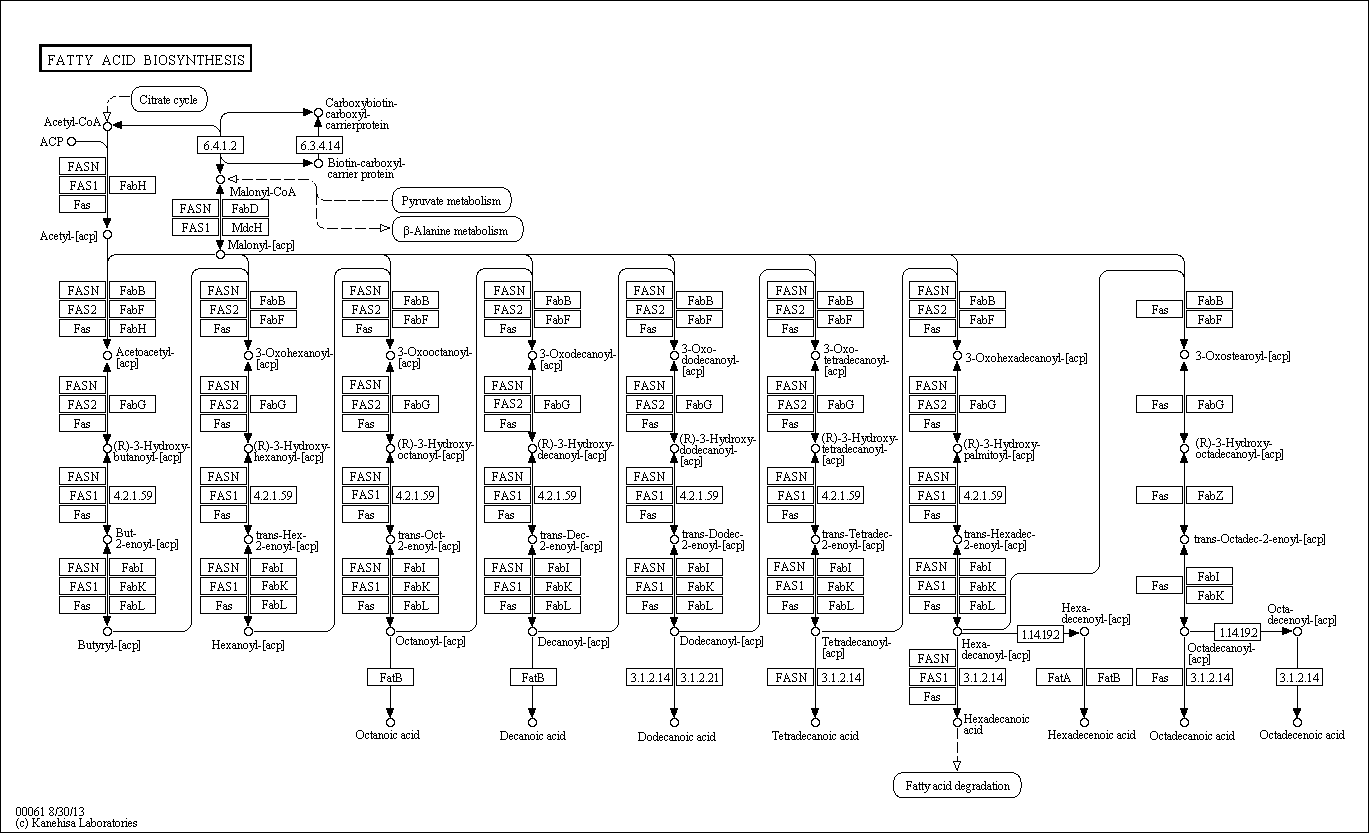
\includegraphics[width=1.0\textwidth]{fa_synthesis_pathway}
\caption[Fatty Acid synthesis pathway]{Fatty acid synthesis pathway
  described by the standard schema in KEGG to capture the component
  iterative pathway of FA synthesis. The working of these
  systems (from experiments for example) is
  integrated with data from multiple sources.}
\label{fig:fa_synthesis_pathway}
\end{figure}

This need to look into dynamic behaviour led to Dynamical System
theory which based on its success in Physics has found its way in many
other fields. Dynamical system theory captures the relationship
between continuous quantities in difference-differential equations
that describe the evolution of state variables in terms of changes
in other state variables and even themselves thus capturing the
interaction element. Since the time of Newton and classical mechanics,
where these ideas originated, the toolbox of dynamical systems theory
has grown to include techniques for qualitative understanding of
system without the need for numerical or analytic solutions.

In biochemistry, each species in the system is represented by its
concentration leading to a differential equation for each species. The
rate of change of the concentration of a species is described in terms
of in-flows (increasing the rate of change/production) and out-flows
(decreasing the rate of change/degradation). These flows can be
dependent on the concentrations of other variables(species) that
participate in the same reaction scheme. Consider, for example, a
system with $n$ components that we can group into the global state of
the system $\mathbf{x} = (x_1, x_2, \dots x_n)$. All the reactions
that take place in the system change, in discrete levels, the numbers
of molecules of the species:

\begin{align*}
\mathbf{x} &\overset{r_1(\mathbf{x})}{\longrightarrow} \mathbf{x} +
\mathbf{\delta_1}\\
\mathbf{x} &\overset{r_2(\mathbf{x})}{\longrightarrow} \mathbf{x} +
\mathbf{\delta_2}\\
\vdots \\
\mathbf{x} &\overset{r_m(\mathbf{x})}{\longrightarrow} \mathbf{x} +
\mathbf{\delta_m}
\end{align*}
So for every reaction we have one such rule and the
discrete levels $\delta_k$ by which the species change for every reaction. Each
reaction has an associated and possible state dependent rate $r_k(x)$
that is the expected number of times it takes place in a
unit of time. The in-flows are the positive deltas and out-flows the negative
ones. The differential equation describing the evolution of the average numbers
of  species $i$ is then the sum of the in- and out- flows
over all reactions in the system:

\begin{equation*}
\frac{dx_i}{dt} = \sum_{m} r_m(\mathbf{x})\delta_{mi}
\end{equation*}

Usually this formulation of the problem leads to integration, with a
numerical ODE solver of the above system to get the dynamic behaviour
of the system. The usual problem mathematical biologists face is that
the reaction rate function (the $r_k(\mathbf{x})$) contain parameter
constants that are not usually known.

In the contex of metabolic systems however, there is a mathematical technique, called Flux Balance
Analysis, that is used to compute these flows without explicit
knowledge of these parameters by making some assumptions about the
system to simplify the problem \cite [] {orth2010flux}. If we assume that that metabolites
cannot accumulate within the cell and their levels are more or less
balanced, then the system is immediately at steady-state. The steady-state assumption means that the average positive flux-defined as the sum of
all the in-flows- and the average negative flux-defined as the sum of
all the out-flows- are equal. This in turn means that the rate of
change for every species, defined as the sum of all flows(negative and
positive), is zero (cancelled). Solving for the fluxes leads to a linear equation for each
species. For a more concise notation, all the $\delta_{nm}$ are
packaged into $\mathbf{S}$, traditionally called the Stoichiometric
matrix, and the fluxes in a vector $\mathbf{r}$. The problem
is reduced to solving the system $\mathbf{Sr} = \mathbf{0}$ to calculate the
fluxes $\mathbf{r}$ through our system of interest. The only problem
with this formulation is that the system is
underdetermined since usually the number of reactions is higher than
the number of species. To solve this, the solution space is constrained
with the use of an objective function that leads to a linear
programming problem formulation that is easily solvable. A small
contrived example to illustrate the above process is given in
Figure~\ref{fig:fba}.

\begin{figure}[htbp!]
\centering
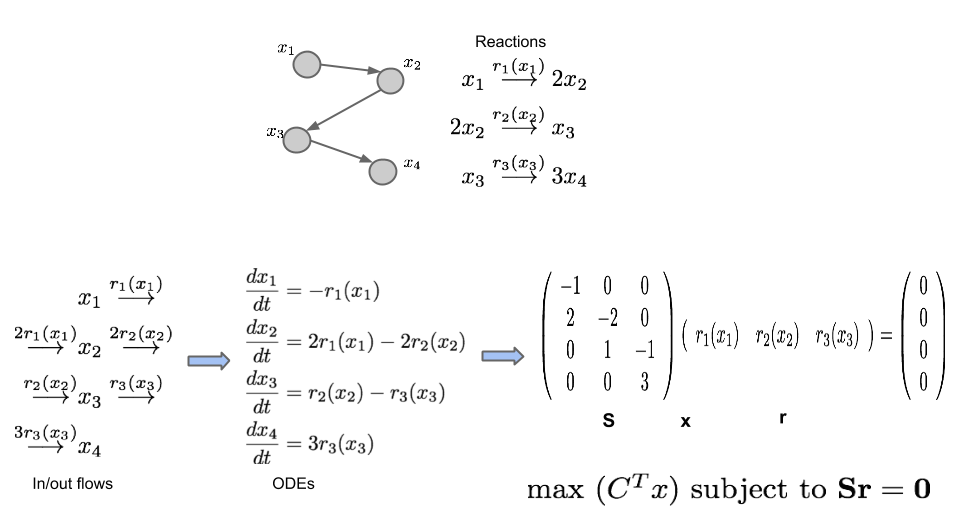
\includegraphics[width=1.0\textwidth]{fba}
\caption[Flux Balance analysis]{A small example how starting from a
  bottom-up model like a pathway from KEGG we can go on to apply FBA
  and calculate the fluxes through our pathway}
\label{fig:fba}
\end{figure}

Flux balance analysis is a very powerful technique since it allows us
to overcome the problem of the rate function parameters and calculate the
fluxes through the system in a computationally efficient way. It is
not without its limitations though. For large networks of components
finding a suitable objective function to used to transform to solve
the underdetermined problem can be difficult. Different objective
functions depend on obserable behaviour based for example on
exponential growth or products of the fermentation process. More importantly and
since it relies on the average behaviour as described by the
differential equations it is not able to capture stochastic,
non-deterministic behaviour.

\section{Challenge of lipid metabolism}
Unlike intermediate metabolism, well-characterised with
stoichiometries per reaction, there are molecules of metabolism that
are poorly annotated, involving iterative chemical processes,
hierarchical processes and non-selective processes. Examples include
Redox Reactions, toxic metabolism, lipid metabolism. Here we try to
capture the latter one.
Lipid metabolism is the set of all the anabolic and catabolic
processes that involve lipid products that serve mainly as energy
stores or in the form of lipid bilayers as membranes. The starting
point of lipid metabolism are the Fatty Acids which act as building
blocks for more complex lipids like diacylglycerols and triacylglycerols. Lipids are
produced by the organism to serve as intracellular compartments and energy stores in the well-fed state when there is an excess
of carbohydrates and no immediate energy requirements. Any excess
glucose molecules are converted to lipids as follows: When the
glucogen stores are full, the carbon from glucose molecules will find its way through
the glycolysis pathway blocked at the level of phosphofructokinase so
they take a diversion through the Pentose Phosphate pathway and then
join the glycolytic processes at a later stage bypassing the
block. Then they continue down the normal route to Acetyl-CoA and the
Krebs cycle in the mitochondria. Here since the immediate energy requirements
are low Acetyl-CoA only makes it to the first stage of the Krebs cycle
producing Citrate instead of continuing through the cycle and then to
the Respiratory chain to produce energy. Since Citrate cannot proceed any further in the
cycle, its levels accumulate and at some point it translocates from
the mitochondrion into the cytosol where it is converted to Acetyl-CoA
again to serve as a precursor to Fatty Acid Synthesis which requires
the NADPH produced by the Pentose Phosphate pathway. Once Fatty Acids
are synthesised they can go on to form more complex lipid products
like DAGs or
TAGs or get further modified by the Fatty Acid elongation pathway or
by adding bonds to their CH tails. The beta-oxidation pathway in
mitochondria breaks down Fatty Acids into Acetyl-CoA which is then fed
into the Krebs cycle \cite [] {salway2013metabolism}.

\begin{figure}[htbp!]
\centering
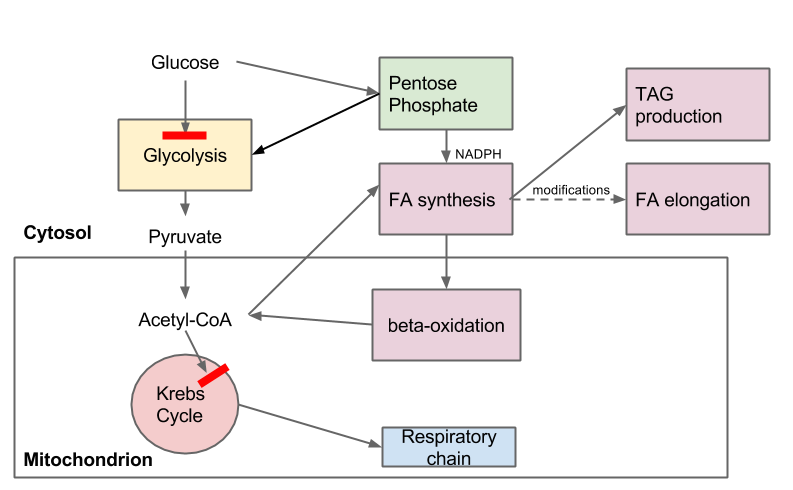
\includegraphics[width=1.0\textwidth]{metabolism}
\caption[Lipid metabolism and interacting pathways]{A diagram
  outlining the main pathways involved in lipid metabolism.}
\label{fig:lipid_metabolism}
\end{figure}

Production processes have equivalent catabolic
processes and a balance between the two is essential for metabolic
homeostasis in organisms. This balance is regulated by control signals
within and
between pathway that also integrate signals from the
environment. In diseases like type 1 Diabetes, this balance is
disrupted because of insulin deficiency that breaks the regulatory
signals. Fatty Acids and lipid metabolism pathways play a key role
in this chain of disruption. Also, free Fatty acids are
associated with obesity and type 2 diabetes \cite [] {boden2002free}.

We notice from the above brief overview and the pictorial description
of the interconnected pathways(Figure~\ref{fig:lipid_metabolism}) that
in metabolism and lipid metabolism products flow through the
network occurs with an iterative chain-like conversion process and that at
several points there are probabilistic decisions to be made for the next step in the
chain. The decisions are tightly regulated by signals from other
pathways and the environment and it is assumed that disruption of these signals is
observed in diseases like Diabetes. It is important therefore to have
a mechanistic explanation of the 'trip' through the metabolic chain
and the non-deterministic 'decision-making' that happens and its regulation. We believe
that in order to get this mechanistic characterisation, we
benefit from a stochastic reaction-centric view of lipid metabolism to
give a more local perspective of the iterative conversion processes
and the stochastic nature of the probabilistic
decision-making process. In this study we
focus on the Fatty Acid Biosynthesis pathway which is an important
part of lipid metabolism. It exhibits the characeteristics that are
suited to a reaction-centric analysis: iterative behaviour with
non-deterministic decisions and regulatory mechanisms from other pathways.

A biochemical system, like the one given in the previous section,
consisting of a number of reactions that alter the integer numbers of
molecules of the species describes a stochastic process and a Continuous
Time Markov Chain (CTMC) in particular. The differential equations we used as
a basis for FBA are just a
deterministic view of the average behaviour. The dynamics of the
system can be set in motion inside a computer using the Gillespie
exact simulation algorithm that creates sample
time-series \cite [] {gillespie1977exact}. Statistical information, like the strength of the
fluctuations (normalised variance) can be computed by collecting a lot
of these traces.

In this study we propose Petri Nets as an alternative language for capturing this
reaction-centric view. We think this is more expressive than the
standard Markov processes formulation. While Petri Nets and their
evolution through their formal operational semantics also describe a
CTMC and are thus equivalent in power with the standard Markov jump
processes. We believe that they possess some characteristics (see next
section and Methods) that makes them useful in the analysis of the
reaction-centric view of lipid metabolism. Language is important not
only because a syntax is needed to define our models but also because
the notation we use is our tool of thought and the use of the correct
language for thinking about a problem can enhance our understadnding
and ultimately help us solving it \cite [] {iverson2007notation}. That is why we have more
than one high-level programming language despite the fact that all of
them are Turing complete and therefore have the ability to express all
computations.

In the next section, we try to place Petri Nets, the main modelling
language used, and pi-calculus, the alternative used as a way to
contrast net and process algebras models, in a spectra of formal
modelling methods for distributed computation.

\section{Computational models in Biology}
Computer Science, although a fundamentally different discipline than
Biology, has undergone a similar transformation in its focus from
single information processing entities to systems of interacting
entities(see the Internet, clusters). The term computation at the
distributed level is now broader; it not only describes mere
calculation but it also includes the interaction between
components. This change in the term computation can be seen through
the models we use to capture the notion of computation. At the early
days of computing(even before actual electronic computers) the models
of computation included lambda-calculus and Turing Machines. These
early formalisms capture computation differently, Turing Machine as
global state transitions in an Abstract Machine and lambda-calculus
as reduction rules in a calculus, but they are effectively equivalent
in expressive power(see Church-Turing thesis). As computer systems
grew there was an interest for similar
minimalistic languages to express distributed computation. Some
formalisms that were invented during that period were
\citet{milner1980calculus} Calculus of Communicating Systems,
\citet{lafont1989interaction} Interaction nets,
\citet{milner1992calculus} pi-calculus, and Petri
Nets \cite [] {murata1989petri}.

The analogy between distributed computer systems and biochemical
systems was made explicit by \citet{berry1989chemical} and the
Chemical Abstract Machine. The modelling langugages used for
distributed computation are applicable in biological systems since
they both include a high number of concurrent components with dependencies
introducing non-deterministic behaviour. \citet{fontana1996barrier} went as far as
to propose pi-calculus as an alternative to dynamical systems
theory since he considered a calculus of objects that can change and their
interactions more appropriate for describing biochemical systems than a calculus of continuous
interacting quantities. \citet{priami2001application} went on to use a
stochastic version of pi-calculus to describe a biochemical systems
and from then other formalisms were developed like
\citet{cardelli2005brane} with Brane-calculi, \citet{danos2004formal}
with kappa, and
\citet{ciocchetta2009bio} with Bio-PEPA.

Petri Nets lean towards the automata and Turing Machines style of
computation because their operational semantics are in terms of state
transitions from a distributed global state. They have a very intuitive
graphical notation and concurrency,
non-determinism, and the causal independencies between events is
inherent in their structure. They
also have a very natural correspondence to biochemical reactions and
in their basic form have been used mainly to capture qualitative properties
of biochemical systems \cite [] {baldan2010petri}. In this study we use the stochastic version of
Petri Nets that explicitly models time to describe and quantitatively
analyse the
reaction-centric view of the FA elongation and synthesis
process.

Process algebras, which pi-calculus is an example of, on the other
hand define syntax to specify the behaviour and state transitions of the individual
components of the system independently therefore reactions and
compositionality are not explicitly captured. In this study we
use Stochastic Pi Machine (SPiM) which is a programming
language derived from stochastic pi-calculus but extended to include
operational semantics for execution on an Abstract Machine and also a
formal graphical notation \cite [] {export:65224, export:65223}. The
fact that this variant shares
characteristics from both net models and process algebras approached
makes it an interesting case-study.

\section{Outline of work}
The main aim of this study was to assess the
applicability of the Petri net formal language to capture a
reaction-centttric view of lipid metabolism by producing a model of the
Fatty Acid biosyntesis/elongation process. For completeness we also
created a stochastic pi-calculus version of the model to contrast the
two methods as part of the more general exploration towards executable
formal models in Biology. An extended version of the basic FA
synthesis model is
also given that includes part of its regulatory mechanisms.

In chapter~\ref{chap:methods} an overview of the methods used in
modelling the process is given, namely Petri Nets and stochastic
pi-calculus. In Section~\ref{chap:work}, the basic and extended model
are presented along with their tuning with available metabolomics
data. 

